 \chapter{Marco Teórico: Álgebra lineal y métodos de factorización matricial}
 \markboth{CAPÍTULO 2. Marco Teórico: Álgebra Lineal y Métodos de Factorización Matricial}{\small CAPÍTULO 2. Marco Teórico: Álgebra Lineal y Métodos de Factorización Matricial}
 \label{MarcoTeorico}

\section{Álgebra lineal}

\noindent El \textbf{álgebra lineal} constituye una rama fundamental de las matemáticas que estudia estructuras como vectores, espacios vectoriales, matrices y transformaciones lineales. Su relevancia trasciende el ámbito teórico, extendiéndose a numerosas aplicaciones en ciencia, tecnología e ingeniería. Representa la base de múltiples técnicas computacionales modernas, desde el análisis numérico hasta el aprendizaje automático, incluyendo el modelado de sistemas físicos, financieros y estadísticos.

Desde una perspectiva educativa, el álgebra lineal frecuentemente representa el primer contacto de los estudiantes con las matemáticas abstractas. La transición desde el álgebra elemental --centrada en ecuaciones y manipulaciones simbólicas-- hacia un pensamiento más estructurado requiere un cambio cognitivo significativo. La abstracción inherente a las matrices, los vectores en espacios de dimensión arbitraria y la interpretación de operaciones como transformaciones lineales puede dificultar el aprendizaje si no se complementa con estrategias pedagógicas adecuadas.

Diversos autores (Dorier, Robert, Robinet \& Rogalski, 2000; Harel \& Kaput, 1991) han señalado que los enfoques tradicionales de enseñanza del álgebra lineal suelen enfatizar excesivamente los procedimientos algebraicos, sin establecer conexiones suficientes con la visualización geométrica, la interpretación conceptual o las aplicaciones prácticas. Como respuesta a esta problemática, se ha impulsado el desarrollo de estrategias didácticas basadas en la interacción, la visualización y la experimentación guiada mediante recursos digitales.

\subsection{Matrices}

Las \textbf{matrices} son arreglos rectangulares de elementos numéricos que permiten representar sistemas lineales, transformaciones entre espacios vectoriales y operaciones algebraicas complejas. Formalmente, una matriz $A \in \mathbb{R}^{m \times n}$ corresponde a un conjunto de elementos reales dispuestos en $m$ filas y $n$ columnas.

Estas estructuras representan el núcleo operativo del álgebra lineal computacional, permitiendo codificar problemas y aplicar algoritmos eficientes. Entre sus operaciones fundamentales destacan la adición, multiplicación, transposición, cálculo del determinante, inversión y reducción por filas, todas ellas esenciales para la solución de sistemas y la implementación de métodos numéricos. Su interpretación geométrica resulta igualmente crucial: cada matriz puede conceptualizarse como una transformación que actúa sobre vectores, modificando regiones del espacio.

\subsection{Determinantes}

El \textbf{determinante} de una matriz cuadrada constituye un valor escalar que sintetiza propiedades fundamentales de la matriz: su invertibilidad, el volumen generado al transformar un espacio y la orientación (preservada o invertida) de dicha transformación. Matemáticamente, si $\det(A) \neq 0$, entonces $A$ resulta invertible y el sistema lineal $Ax = b$ posee solución única.

Aunque el cálculo directo de determinantes no resulta eficiente para matrices de gran dimensión, sigue siendo una herramienta esencial para el análisis teórico. Particularmente, las condiciones de aplicabilidad de ciertos métodos de factorización --como Cholesky o LU sin pivoteo-- dependen de que determinados determinantes parciales (menores principales) sean distintos de cero.

\subsection{Sistemas de ecuaciones lineales}

Los \textbf{sistemas de ecuaciones lineales} surgen de la necesidad de resolver simultáneamente un conjunto de ecuaciones algebraicas lineales de la forma:

\[
\begin{aligned}
	a_{11}x_1 + a_{12}x_2 + \cdots + a_{1n}x_n &= b_1 \\
	a_{21}x_1 + a_{22}x_2 + \cdots + a_{2n}x_n &= b_2 \\
	\vdots \quad \quad \quad & \vdots \\
	a_{m1}x_1 + a_{m2}x_2 + \cdots + a_{mn}x_n &= b_m \\
\end{aligned}
\]

Este sistema puede expresarse en notación matricial como $A\mathbf{x} = \mathbf{b}$, donde $A \in \mathbb{R}^{m \times n}$ es la matriz de coeficientes, $\mathbf{x} \in \mathbb{R}^n$ el vector de incógnitas y $\mathbf{b} \in \mathbb{R}^m$ el vector de términos independientes.

Los métodos de solución se clasifican en dos categorías principales:

\begin{itemize}
	\item \textbf{Métodos directos}: Incluyen la eliminación gaussiana, la inversión matricial y las factorizaciones LU, $LL^{\mathrm{T}}$ y $LDL^{\mathrm{T}}$.
	
	\item \textbf{Métodos iterativos}: Comprenden los métodos de Jacobi, Gauss-Seidel y gradiente conjugado, particularmente adecuados para sistemas dispersos o de gran escala.
\end{itemize}

Este proyecto se centra específicamente en los métodos directos basados en factorización matricial, debido a su eficiencia computacional, estabilidad numérica y estructura clara, características que además facilitan su representación didáctica mediante visualizaciones interactivas.

\section{Métodos de Factorización Matricial}

\subsection{Introducción}

La \textbf{factorización matricial} consiste en descomponer una matriz dada $A \in \mathbb{R}^{n \times n}$ en un producto de matrices con estructuras particulares (triangulares, diagonales, ortogonales, entre otras). Esta descomposición facilita:

\begin{itemize}
	\item La resolución de sistemas de ecuaciones lineales
	\item El cálculo de matrices inversas y determinantes
	\item La implementación de métodos numéricos avanzados
\end{itemize}

Desde una perspectiva didáctica, el proceso de factorización permite a los estudiantes:

\begin{itemize}
	\item Analizar la estructura interna de las matrices
	\item Comprender las transformaciones paso a paso
	\item Visualizar la contribución de cada componente en la solución del sistema
\end{itemize}

En las siguientes secciones se detallan tres métodos fundamentales que serán implementados en el software interactivo.

\subsection{Factorización LU}

La \textbf{factorización LU} constituye una técnica fundamental del álgebra lineal numérica que descompone una matriz cuadrada $A$ como el producto:

\[
A = LU
\]

donde:
\begin{itemize}
	\item $L$ es una \textbf{matriz triangular inferior} ($l_{ij} = 0$ para $j > i$)
	\item $U$ es una \textbf{matriz triangular superior} ($u_{ij} = 0$ para $i > j$)
\end{itemize}

\subsubsection{Aplicación a sistemas lineales}

Para resolver el sistema $A\mathbf{x} = \mathbf{b}$, la factorización LU permite:

\begin{enumerate}
	\item \textbf{Sustitución progresiva}: Resolver $L\mathbf{y} = \mathbf{b}$
	\item \textbf{Sustitución regresiva}: Resolver $U\mathbf{x} = \mathbf{y}$
\end{enumerate}

Esta descomposición ofrece ventajas significativas:

\begin{itemize}
	\item Eficiencia computacional al resolver múltiples sistemas con la misma matriz $A$
	\item Modularización del proceso de solución
	\item Claridad conceptual para fines didácticos
	\item Facilidad de implementación algorítmica
\end{itemize}

%\begin{observacion}
	La factorización LU existe y es única si y solo si todos los menores principales de $A$ son no singulares.
%\end{observacion}

\subsection{Variantes de la factorización LU}

Existen dos variantes principales de la factorización LU, diferenciadas por la normalización de los elementos diagonales:

\subsubsection{Factorización de Doolittle}

La factorización de Doolittle se caracteriza por:

\begin{itemize}
	\item Matriz $L$ con \textbf{unos en la diagonal principal}
	\item Matriz $U$ con los coeficientes completos en la parte superior
\end{itemize}

\[
L = \begin{bmatrix}
	1 & 0 & 0 \\
	l_{21} & 1 & 0 \\
	l_{31} & l_{32} & 1
\end{bmatrix}, \quad
U = \begin{bmatrix}
	u_{11} & u_{12} & u_{13} \\
	0 & u_{22} & u_{23} \\
	0 & 0 & u_{33}
\end{bmatrix}
\]

\subsubsection{Factorización de Crout}

La factorización de Crout presenta:

\begin{itemize}
	\item Matriz $U$ con \textbf{unos en la diagonal principal}
	\item Matriz $L$ con todos los coeficientes multiplicadores
\end{itemize}

\[
L = \begin{bmatrix}
	l_{11} & 0 & 0 \\
	l_{21} & l_{22} & 0 \\
	l_{31} & l_{32} & l_{33}
\end{bmatrix}, \quad
U = \begin{bmatrix}
	1 & u_{12} & u_{13} \\
	0 & 1 & u_{23} \\
	0 & 0 & 1
\end{bmatrix}
\]

%\begin{observacion}
	Ambas factorizaciones son matemáticamente equivalentes en términos de su aplicación. La elección entre ellas depende de consideraciones algorítmicas y pedagógicas. La variante de Doolittle suele preferirse en contextos educativos por su directa relación con el proceso de eliminación gaussiana.
%\end{observacion}

\subsection{Relevancia pedagógica de la factorización LU}

La factorización LU ofrece importantes ventajas didácticas en la enseñanza del álgebra lineal:

\begin{itemize}
	\item \textbf{Proceso constructivo}: Permite visualizar la transformación gradual de la matriz original $A$ en las matrices $L$ y $U$, reforzando la comprensión de la eliminación gaussiana.
	
	\item \textbf{Estructura transparente}: Facilita la identificación de los multiplicadores gaussianos en $L$ y los coeficientes resultantes en $U$.
	
	\item \textbf{Detección de errores}: La escritura manual de las matrices ayuda a reconocer y corregir errores frecuentes en la disposición de los elementos.
	
	\item \textbf{Aplicación sistemática}: Proporciona un método general para resolver sistemas lineales, con especial relevancia en:
	\begin{itemize}
		\item Matemáticas aplicadas
		\item Ingeniería
		\item Ciencias computacionales
	\end{itemize}
\end{itemize}

%\begin{teorema}
	La factorización LU existe para una matriz $A \in \mathbb{R}^{n \times n}$ si y solo si todos sus menores principales son no singulares.
%\end{teorema}

La combinación de \textbf{estructura clara} y \textbf{aplicaciones prácticas} convierte a la factorización LU en una herramienta fundamental para vincular los conceptos teóricos con su implementación algorítmica.


\subsection{Consideraciones numéricas y estrategias de pivoteo}

En la implementación práctica de la factorización LU, especialmente al trabajar con matrices mal condicionadas o con elementos pivote nulos, es fundamental garantizar la \textbf{estabilidad numérica} del algoritmo. Esta estabilidad se consigue mediante la técnica de \textbf{pivoteo parcial}, que reorganiza las filas de la matriz original mediante una matriz de permutación:

\[
PA = LU
\]

donde:
\begin{itemize}
	\item $P$ es una \textbf{matriz de permutación} que codifica los intercambios de filas realizados
	\item $L$ mantiene su estructura triangular inferior con unos en la diagonal
	\item $U$ conserva su forma triangular superior
\end{itemize}

El pivoteo parcial ofrece dos ventajas principales:
\begin{enumerate}
	\item Evita divisiones por cero al seleccionar el elemento de mayor magnitud como pivote
	\item Minimiza la propagación de errores de redondeo en cálculos numéricos
\end{enumerate}

%\begin{observacion}
	En el diseño de herramientas educativas, el módulo de pivoteo parcial puede implementarse como \textbf{contenido avanzado}, accesible únicamente después de que los estudiantes hayan asimilado la versión básica de la factorización LU.
%\end{observacion}

\subsection{Especificaciones del programa interactivo}

El sistema educativo deberá incorporar las siguientes funcionalidades clave para facilitar el aprendizaje de la factorización LU:

\begin{enumerate}
	\item \textbf{Módulo de entrada de datos}
	\begin{itemize}
		\item Interfaz gráfica para ingreso manual de matrices
		\item Generación automática de matrices con diferentes propiedades
		\item Importación desde archivos externos
		\item Validación automática de dimensionalidad y propiedades matriciales
	\end{itemize}
	
	\item \textbf{Visualización interactiva}
	\begin{itemize}
		\item Representación animada del proceso de eliminación gaussiana
		\item Actualización dinámica de los elementos de $L$ y $U$
		\item Resaltado gráfico de las operaciones en curso
		\item Control de velocidad y pausa para análisis detallado
	\end{itemize}
	
	\item \textbf{Sistema de evaluación}
	\begin{itemize}
		\item Ejercicios guiados para completar elementos de las matrices
		\item Retroalimentación inmediata con explicaciones detalladas
		\item Registro histórico de intentos y progreso
		\item Mecanismo de ayuda gradual tras múltiples intentos fallidos
	\end{itemize}
	
	\item \textbf{Análisis comparativo}
	\begin{itemize}
		\item Visualización simultánea de las variantes Doolittle y Crout
		\item Análisis de estabilidad numérica para diferentes matrices
		\item Comparación de rendimiento computacional
	\end{itemize}
	
	\item \textbf{Resolución de sistemas lineales}
	\begin{itemize}
		\item Implementación completa del proceso de solución
		\item Visualización de las sustituciones progresiva y regresiva
		\item Verificación numérica de las soluciones obtenidas
	\end{itemize}
	
	\item \textbf{Recursos pedagógicos}
	\begin{itemize}
		\item Explicaciones contextuales adaptadas al nivel del usuario
		\item Catálogo de errores frecuentes con sugerencias de corrección
		\item Diccionario matemático integrado
		\item Ejemplos resueltos paso a paso
	\end{itemize}
	
	\item \textbf{Características avanzadas}
	\begin{itemize}
		\item Exportación de resultados en formatos estándar
		\item Implementación de pivoteo parcial
		\item Soporte para matrices dispersas (implementación futura)
		\item Personalización de parámetros numéricos
	\end{itemize}
\end{enumerate}

%------------------------------------------------------------------------------------------------------------
\section{Nombre de la sección}\label{EtiquetaDeSeccion21}
\noindent
\begin{thm}
	Enunciado del teorema
\end{thm}

\begin{cor}
	Enunciado del corolario
\end{cor}

\begin{lem}
	Enunciado del lema
\end{lem}

\begin{obs}
	Enunciado de la observación
\end{obs}


%------------------------------------------------------------------------------------------------------------
\section{Ejemplo para referenciar figuras y tablas}\label{EtiquetaDeSeccion22}
\noindent Se puede observar en la Figura \ref{EtiquetaFigura} ...
\begin{figure}[h!]
	\caption{Gráfica de la función $f(x,y)=\frac{\sin{\sqrt{x^2+y^2}}}{x^2+y^2}$}
	\centering
	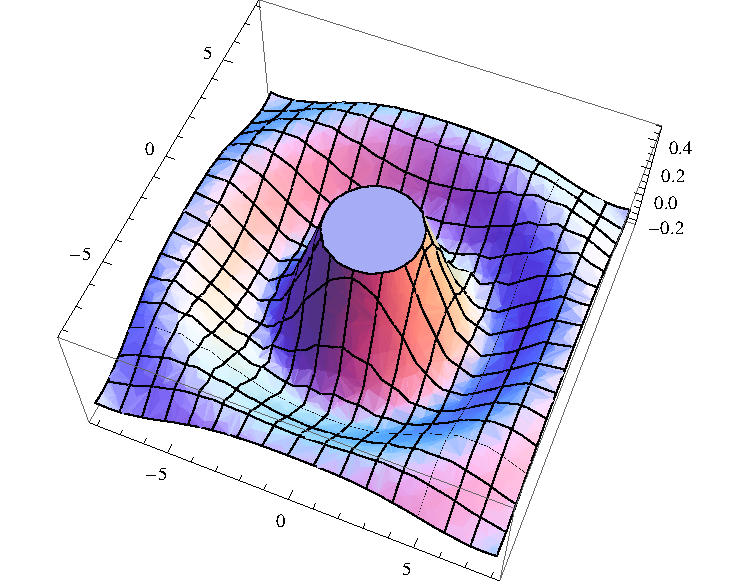
\includegraphics[width=7cm]{EjemploFigura.pdf}
	\label{EtiquetaFigura}
	\medskip
	\caption*{\emph{Nota}: Esta es una nota explicativa\\ sobre la imagen (opcional)}
\end{figure}

\noindent En la Tabla \ref{EtiquetaDeLaTabla} ...
\begin{table}[h!]
\caption{Título de la tabla}
\centering
\begin{tabular}{c|c|c}
	& 1 & 2 \\
	\hline
	A &  &  \\
	\hline
	B &  &  \\
\end{tabular}
\label{EtiquetaDeLaTabla}
\medskip
\caption*{\emph{Nota}: Nota de la tabla (opcional)}
\end{table}


\section{Cómo citar}\label{EtiquetaDeSeccion23}
\begin{itemize}
	\item \textbf{Citas cortas} (hasta 40 palabras):Se incluyen en el texto con comillas.
	\item \textbf{Citas largas} (más de 40 palabras): Se escriben en párrafo separado sin comillas.
\end{itemize}

\subsection{\emph{apacite}}
\noindent Para citar en formato APA, puede usarse el paquete \emph{apacite}. Algunas opciones de citación pueden hacerse con los comandos que se presentan en la Tabla \ref{ComandosApacite}; puede consultar \cite{meijer2013apacite} para la información completa de la documentación del paquete.

\begin{table}[h!]
\caption{Algunos comandos del paquete \emph{apacite} }
\centering
\scriptsize
	\begin{tabular}{ll}
		\hline
		\textbf{Texto plano}&\textbf{Produce}\\
		\hline
		\verb|\cite{RudinKEY} afirma que|&\cite{RudinKEY} afirma que \\
		\verb|\cite[p.123]{RudinKEY} afirma que|&\cite[p.123]{RudinKEY} afirma que\\
		\verb|Como se pude ver en  \citep{RudinKEY}|&Como se pude ver en  \citep{RudinKEY}\\
		\verb|\citealp{RudinKEY}|&\citealp{RudinKEY}\\
		\verb|Ver Rudin \citeyearpar {RudinKEY}|&Ver Rudin \citeyearpar {RudinKEY}\\
		\verb|Como se pude ver en  \citet{RudinKEY}|&Como se pude ver en  \citet{RudinKEY}\\
		\verb|Como se pude ver en  \citetext{RudinKEY}|&Como se pude ver en  \citetext{RudinKEY}\\
		\verb|Puede consultar \citeauthor {RudinKEY}|&Puede consultar \citeauthor {RudinKEY}\\
		\verb|Confrontar Lamport \citeyear {RudinKEY}|&Confrontar Lamport \citeyear {RudinKEY}\\
		\hline
	\end{tabular}
\label{ComandosApacite}
\medskip
\caption*{\emph{Nota}: Tabla extraída de \citet[p. 50]{WunschKEY}.}
\end{table}

\subsection{Citas textuales}

\begin{itemize}
  \item \textbf{Narrativa}.

  \underline{Cita corta}.

   Como menciona \cite{apostol1976analisis}, ``\emph{la idea de expresar geométricamente los números complejos como puntos de un plano fue formulada por Gauss en su disertación de 1799 e, independiente, por Argand en 1806.}'' (p. 21). Sin embargo ...

  \underline{Cita larga}

  Como menciona \cite{apostol1976analisis}:
  \begin{itemize}
    \item [] La idea de expresar geométricamente los números complejos como puntos de un plano fue formulada por Gauss en su disertación de 1799 e, independiente, por Argand en 1806. Más tarde Gauss ideó la expresión un tanto desafortunada de ''número complejo''. Los números complejos admiten otras representaciones geométricas. En vez de utilizar puntos de un plano, se pueden utilizar puntos de otras superficies. (p. 22)
  \end{itemize}



  \item \textbf{Con paréntesis}.

  Los números complejos, pueden representarse como puntos de un plano, ``\emph{la idea de expresar geométricamente los números complejos como puntos de un plano fue formulada por Gauss en su disertación de 1799 e, independiente, por Argand en 1806.}'' \cite[p. 21]{apostol1976analisis},

\end{itemize}

\subsection{Citas parafraseadas}
\begin{itemize}
  \item \textbf{Narrativa}.

  De acuerdo a \cite{apostol1976analisis}, otra representación geométrica de los números complejos es la llamada \textbf{proyección estereográfica} que consiste en proyectar los puntos del polo norte de la esfera sobre el plano tangente en el polo de dicha esfera. (p. 22)
  \item \textbf{Con paréntesis}.

  Otra representación geométrica de los números complejos es la llamada \textbf{proyección estereográfica} que consiste en proyectar los puntos del polo norte de la esfera sobre el plano tangente en el polo de dicha esfera.\cite[p. 22]{apostol1976analisis}
\end{itemize}



